One desired feature was the ability to automatically generate usable milestone documentation entirely from model elements. Historically, students took screenshots of diagrams and exported lists of requirements to Microsoft Excel to edit, manipulate, and format for usage in formal documents. This has proven to be a problematic process. For example, once a team member exports a subsystem requirement list to Excel, the source of truth becomes that Excel sheet, requiring the team lead to always compare the names, IDs, and details of requirements between different documents. The CubeSat model previously used in AFIT's first spacecraft design course provided a starting point to determine which model elements were important for the key documents in the early stages of a system design. This model featured package diagrams with views and viewpoints pointing to model elements, and used the "Document Preview" plugin to pull model elements into an html file. Figure \ref{fig:CONOPS Document Generator} shows one small piece of the document generator for the \abbreviationFull[Concept of Operations]{CONOPS}, and Figure \ref{fig:CONOPS Document Generator Output 2} show what this plugin displayed as the output. 

\begin{figure}
    \centering
    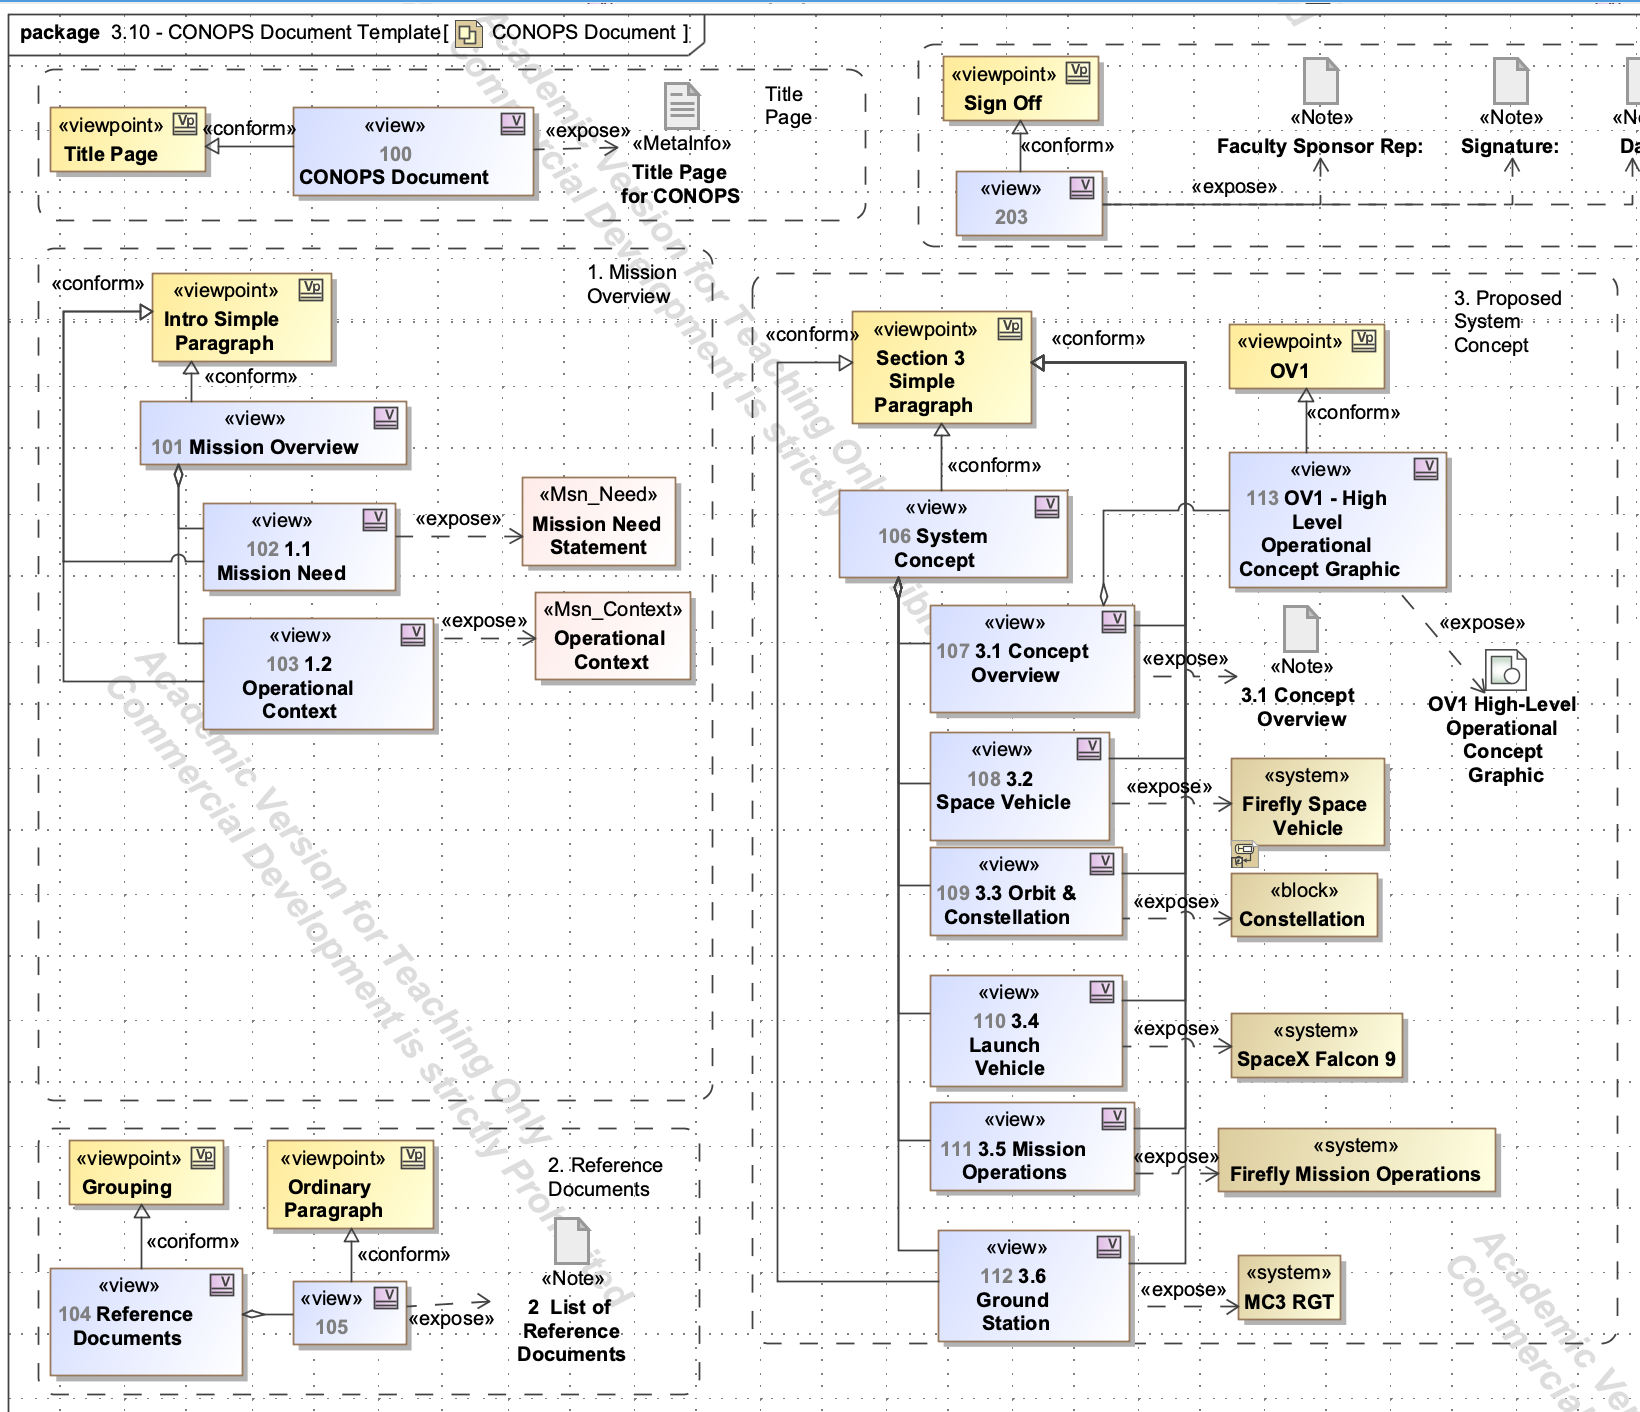
\includegraphics[width=\textwidth]{Thesis/Literature_Review/Lit Review Figures/ayres document generator.png}
    \caption{CONOPS Document Generator}
    \label{fig:CONOPS Document Generator}
\end{figure}

\begin{figure}
    \centering
    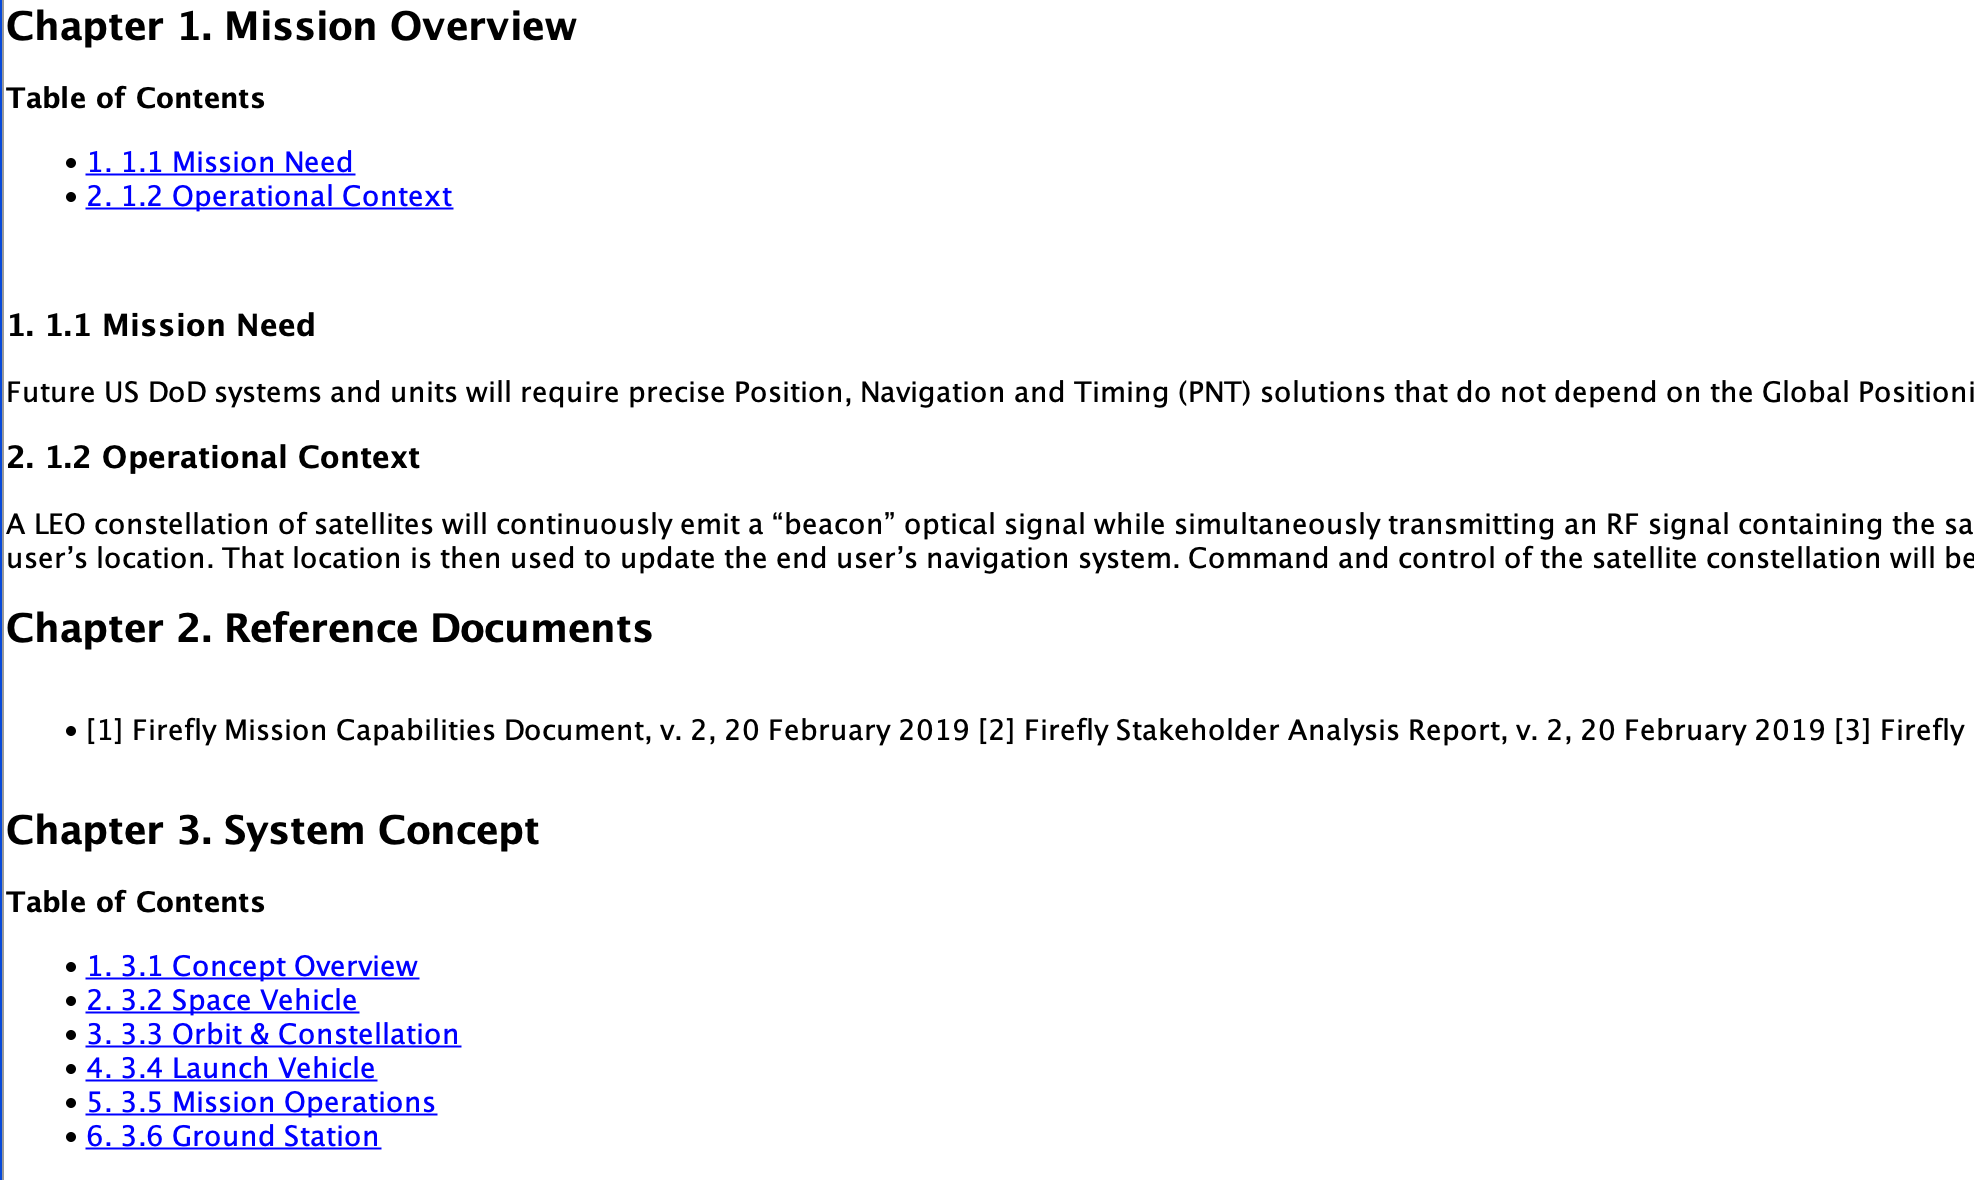
\includegraphics[width=\textwidth]{Thesis/Literature_Review/Lit Review Figures/old method of doc generator 2.png}
    \caption{CONOPS Document Generator Output}
    \label{fig:CONOPS Document Generator Output 2}
\end{figure}

This was a useful start, as it used model elements to generate documentation, but there were several issues with this method. First, this plugin has been unreliable. Most students have trouble getting it to work at all, and the pdf functionality seems to be broken in recent versions of Cameo. As shown in Figure \ref{fig:CONOPS Document Generator Output 2}, the numbering and organization was quite frustrating to deal with. The document generator was difficult to tweak, as it determined the document order based off view and viewpoint IDs, not based on the layout of the diagram or any other easy way to reorganize or add new elements to. Figure \ref{fig:CONOPS Document Generator Output 2} shows that the html file pulled text from the model, but customization and formatting was poor. In practice, users had to just copy and paste this html file into Microsoft Word and then spend a lot of time properly formatting it so that it was presentable and properly formatted and polished. Any changes to the model required all this work to be done over again unless the user wanted to individually copy and paste text from the model for the document. Finally, this is a plugin in beta, and seems to be unavailable for the latest service pack of Cameo. These were useful though to determine the content and order of each document, but this thesis will propose a different solution for generating documents. 